\documentclass[12pt]{article}
\usepackage{graphicx}
\usepackage{wrapfig}
\usepackage[colorlinks=true,urlcolor=blue]{hyperref}
\usepackage{xcolor}
\usepackage{listings}
\usepackage{caption}
\graphicspath{ {./images/} }

\title{A Guide To Linux for University of Toronto Undergraduate Physics Students}
\author{Yigit Ozcelik 2T3}
\date{\today}

\begin{document}
\maketitle

\pagebreak
\tableofcontents

\pagebreak
\section*{Introduction}

\subsection*{What Is This?}

This document is a guide to what Linux is and how to use it for the purposes of academic writing and scientific computing. It is aimed primarily at undergraduate physics students at the University of Toronto, where the author obtained his degree in physics in 2023. 

This document will introduce you to Linux, make a case for why you might want to use it, describe how to install and use a Linux operating system on your computer (or in a virtual machine), introduce you to some fundamental Linux concepts (the terminal, package managers, etc.), and then focus on setting up important tools for a physicist-in-training at UofT (such as a Python coding environment and a LaTeX setup). 

\subsection*{What Is Linux?}

Linux is an \textbf{operating system-} an operating system (`OS') is responsible for managing the interactions between hardware and the other software running on the computer. Linux serves as an alternative to Mac OS or Windows. 

However, there are several fundamental differences between Linux and Windows/Mac OS. Here are a few:

\textbf{Linux has `distributions'.} Essentially, Linux is very modular; you can modify even the most fundamental parts of Linux. This has led to different versions of Linux being created by different projects to serve different needs and priorities. These different versions are called \textbf{Linux distributions,} or \textbf{Linux distros} for short. Different distros come with different preinstalled programs, different looks (`desktop environments'), different update schedules and so on. Some distros are Ubuntu, Fedora, Arch Linux and Gentoo.

\textbf{Linux is `free' open source software.} Open source software refers to software whose source code is publicly available - you can use the source code to examine or modify the program, including compiling it yourself. `Free' software in this context ( also called `libre software') refers to software that you can use for any purpose, including commercial purposes. Software that is both free and open source is called FOSS (Free and Open Source Software) for short. 

Crucially, the \textbf{Linux kernel,} the core of a Linux OS, is FOSS. This means that anyone (including you!) can build an OS around the Linux kernel, for any purpose, for free - and you can access and edit the kernel's source code to do so. This renders Linux far more versatile than both Windows and Mac OS (which are very much not FOSS). 

\textbf{Linux focuses on using the terminal, rather than graphical applications.} A terminal is a program that lets you execute commands on your computer using text prompts. These commands can both execute text-based programs - meant to be used within a terminal (such as \verb|cd|) - and graphical programs (e.g. the \verb|libreoffice| command runs the graphical LibreOffice program). 

A \textbf{graphical program} here refers to a program that creates a window on the screen - this is likely the case for almost all programs you interact with regularly. In contrast, a \textbf{text program} is accessed through a terminal. 

A great part of the power of a Linux system comes from how terminal commands are deeply integrated into the operating system. You can use text commands in the terminal to manipulate files, run text-based programs, update programs (see below) and to do a million other things that might be cumbersome or downright unfeasible to do in a graphical program.

\textbf{Linux uses `package managers'.} The vast majority of programs installed on a Linux machine are managed (tracked, (re)installed, updated and removed) by a program called a `package manager'. A `package' in this context means `a bunch of files, possibly including programs'. You can think of a package manager as an app store of sorts, where all files and programs you need are bundled into various packages. 

A Linux distribution almost always comes with a package manager, such as \verb|apt| or \verb|pacman|. The package manager used by a distribution is very important - it influences how and where you install packages, for example. Different package managers also take different types of commands.


\subsection*{Why Use Linux?}

There are a large variety of reasons to use Linux. Many servers and various devices around the world use the Linux kernel as a base for their operating systems. Linux operating systems are reliable, quite secure and give you full control of your system. Linux is very customizable, so you can use it in a lot of different scenarios (servers, lightweight installations, and so on).

Furthermore, Linux's focus on FOSS means that most Linux software is free to use, in sharp contrast to most Windows and Mac OS apps. The vast majority of Linux distributions are completely free of charge to download and use.

For our purposes (scientific computing), learning Linux and command line tools will let you effectively manipulate data, easily install Python and similar software, interface with computer clusters during research, and do many other things without worrying about, say, a Windows update interrupting your workflow.

As you read on through the rest of this guide, I hope you will find your own reasons for switching to Linux as well.

\subsection*{Why NOT use Linux?}

There are some factors to consider before committing to installing Linux on your computer (or a virtual machine) - unfortunately, as with any large-scale software, Linux operating systems do have their drawbacks.

Most notably, a lot of proprietary software (Adobe suite, Microsoft Office, most video games) is not available officially for Linux. There are open source alternatives to these, of course (GIMP replaces Photoshop, Libreoffice replaces Word, Steam Proton lets you play most video games), but this can be an obstacle to using Linux as your daily operating system.

Another thing to consider is that Linux is a paradigm shift from more common operating systems. What I mean by the phrase `paradigm shift' is that getting started with Linux is a learning and adaptation process. Especially early on, you will need to do a lot of research and troubleshooting to get things working the way you want them to. (The flipside to this is that there usually \textit{is} a way to get things working exactly how you want!)

\pagebreak
\section{Getting Started: Installing Ubuntu}

\subsection{Ubuntu?}

Ubuntu is generally regarded as the most popular Linux distribution, especially for beginners. There is a colossal community of Ubuntu users out there, full of people who have had the same questions as you. This is the most important asset a beginner-friendly distribution could have. As such, I will be using the most recent version of Ubuntu (at the time of writing) in this guide. That version is \textbf{Ubuntu 23.10} - the version number stands for October 2023.

\subsection{Where should I install Ubuntu?}

You can install Ubuntu in a few ways. Most importantly, you can either directly install Ubuntu onto your hard drive (a `bare metal' install) or you can install Ubuntu into a \textbf{virtual machine-} a program that acts like a computer within your computer.

The latter option is much safer and tidier in terms of learning the ropes. I would only recommend installing Ubuntu to a hard drive if you are using a spare computer (e.g. an old laptop) - if you choose to do so, \textbf{back up all of the data on your computer onto a separate hard drive!} It is possible to mess up to such a degree that completely reinstalling Ubuntu is easier than fixing the issue manually - reinstalling Ubuntu might even be the only reliable solution! Reinstalling Ubuntu on a virtual machine is much safer and easier than reinstalling Ubuntu to a hard drive.

We will be installing Ubuntu into a virtual machine in this guide. 

\subsection{VirtualBox}

The virtual machine software I have decided to use is \textbf{VirtualBox,} which you can download from \url{https://www.virtualbox.org/wiki/Downloads} . Just go to this URL and download the appropriate file for your `host' system (i.e. the operating system of your actual computer), and then follow the instructions in the setup.

Once you have installed VirtualBox, you can proceed to installing Ubuntu into VirtualBox.

\subsection{Downloading Ubuntu 23.10 and Installing into VirtualBox}

Navigate to \url{https://ubuntu.com/download/desktop} and scroll down. Under the ``Ubuntu 23.10" section, click the button labeled ``Download 23.10". This will download the file \verb|ubuntu-23.10.1-desktop-amd64.iso|  \footnote{Here, `amd64' refers to the system architecture of your computer. Carry on with the instructions even if your file name is slightly different.} .

\begin{figure}[htp]
    \centering
    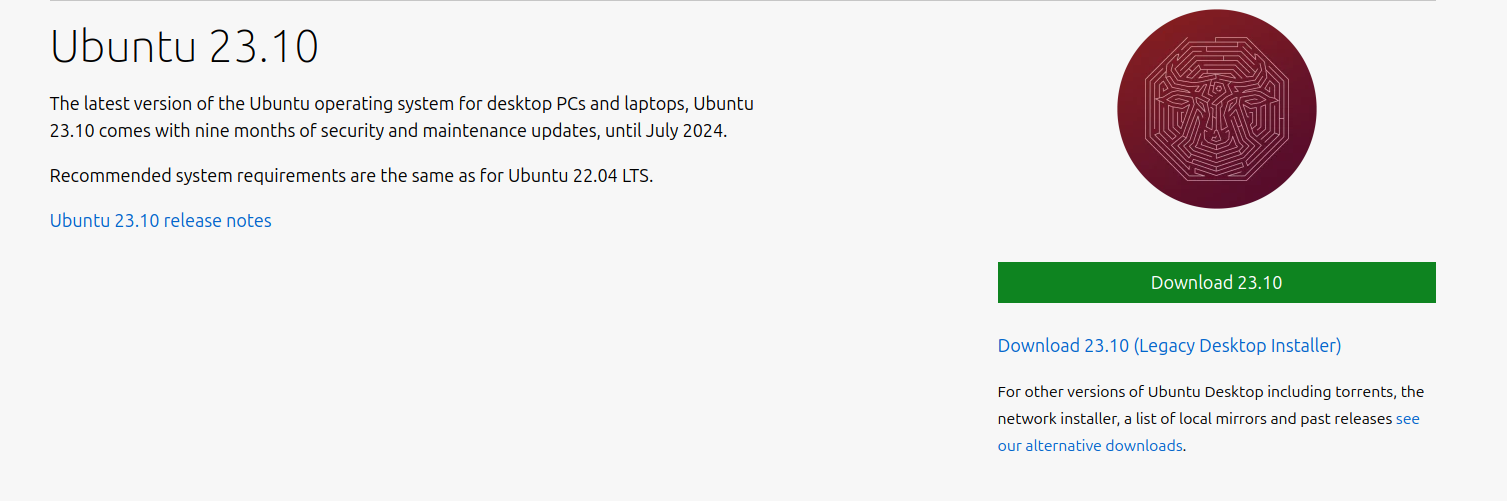
\includegraphics[width=\textwidth]{1-1.png}
\end{figure}

Once the \verb|.iso| file is downloaded, open VirtualBox.

\begin{figure}[htp]
    \centering
    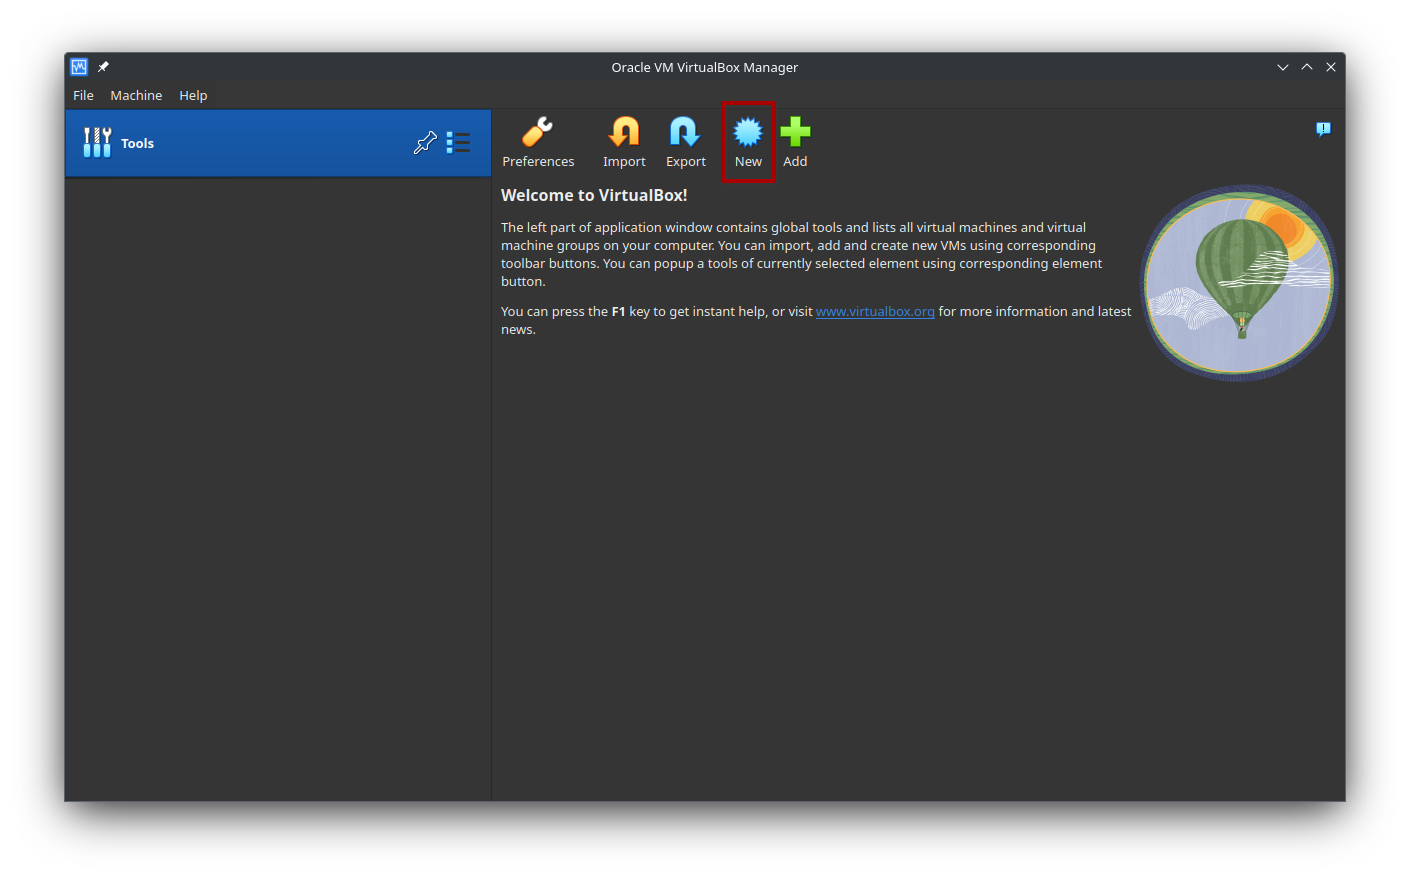
\includegraphics[width=\textwidth]{1-2.png}
\end{figure}

You can create a virtual machine in a few ways in VirtualBox - we will be creating one from the \verb|.iso| file we downloaded earlier. To do so, click ``New" on the icon toolbar (see figure above). A dialog box will appear (see below). \vspace{5mm}

\textbf{Sidebar:} We chose the ``New" option because \verb|.iso| file we downloaded is not the Ubuntu operating system itself - it is an \textbf{installation medium,} which we will use to install Ubuntu proper into a virtual machine\footnote{If you are installing Ubuntu directly to a hard drive, you will need to flash this file to a USB drive and boot your computer from that USB drive. The instructions to do this vary slightly between different computer brands and models.}.\vspace{5mm}

Back to installation. When you click ``New", the dialog box that opens will have several fields we need to fill.

\begin{figure}[htp]
    \centering
    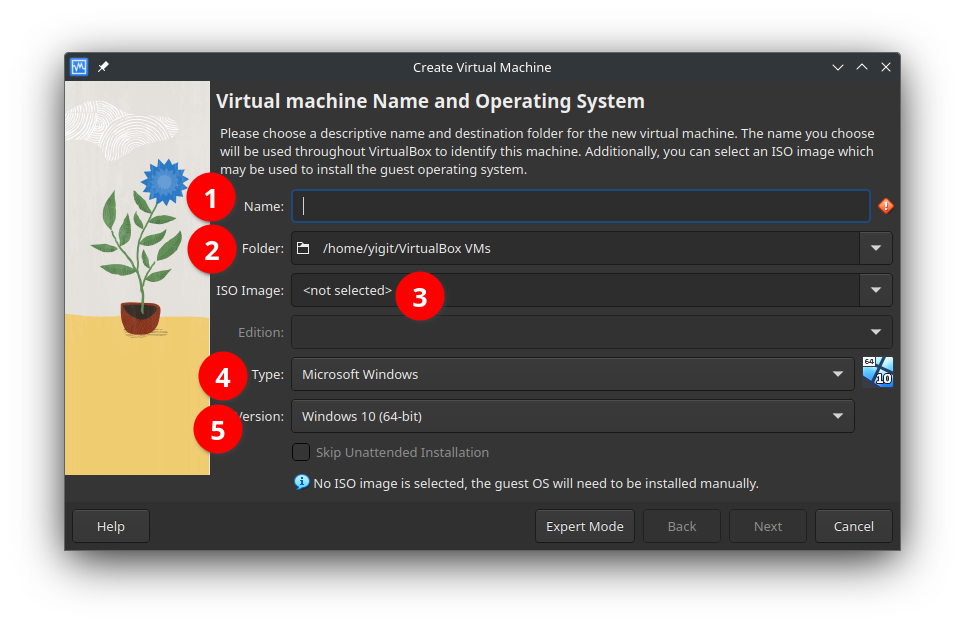
\includegraphics[width=\textwidth]{1-3.png}
\end{figure}

\begin{enumerate}
    \item \textbf{Name:} Enter a name of your choice for the virtual machine.
    \item \textbf{Folder:} Choose the folder where the virtual machine will be created. I recommend creating a dedicated folder for this purpose.
    \item \textbf{ISO Image:} You need to point VirtualBox to the installation medium. Click the drop-down arrow on the right-hand side of this field, select ``Other..." and then find the \verb|.iso| file you downloaded earlier in the file picker.
    \item \textbf{Type:} This will be automatically set to ``Linux" when you select the ISO.
    \item \textbf{Version:} This will be automatically set to ``Ubuntu (64-bit)" when you select the ISO.
\end{enumerate}

Check the ``Skip Unattended Installation" box. We will install the ``guest OS" (Ubuntu) manually\footnote{The unattended installation feature lets you input several extra settings in VirtualBox and then skip Ubuntu's own install dialogue. Although I have opted not to use this feature in this guide (as it is relatively new), you can try it if you wish.}.

\begin{figure}[htp]
    \centering
    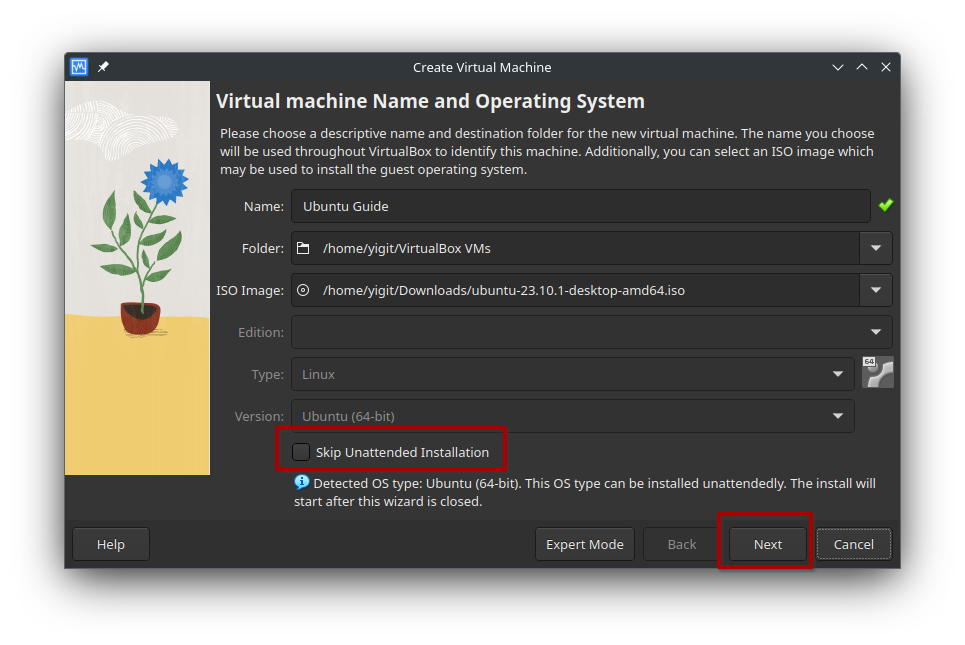
\includegraphics[width=\textwidth]{1-4.png}
\end{figure}

When you are done, click ``Next".

\pagebreak

VirtualBox allocates a certain amount of your computer's memory and CPU resources to the virtual machine when it is running. 

\begin{figure}[htp]
    \centering
    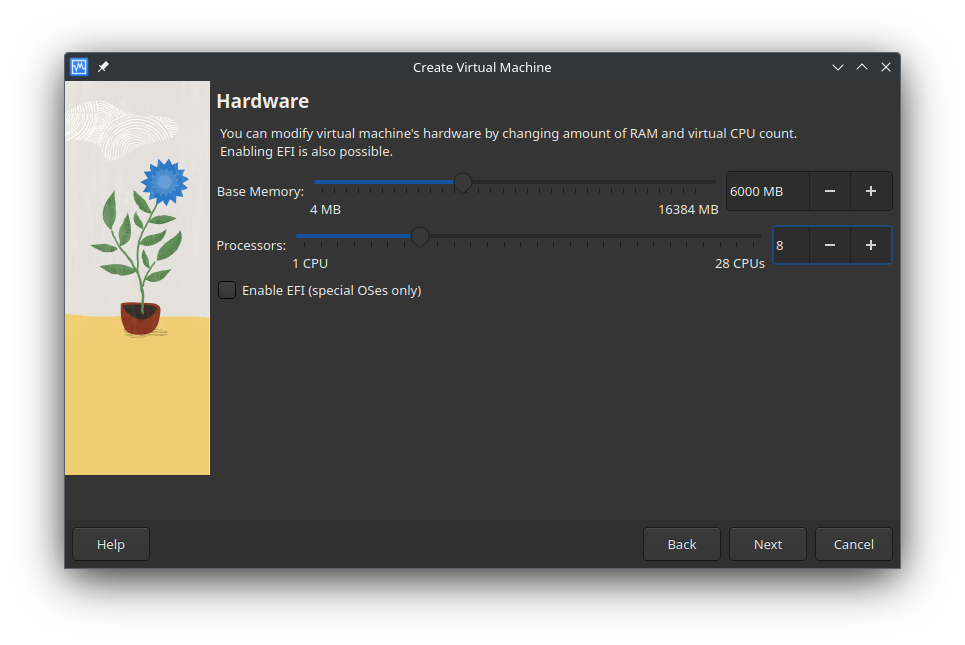
\includegraphics[width=\textwidth]{1-6.png}
\end{figure}

The appropriate amount to choose depends on your hardware; here, I have chosen to allocate 6GB of memory and 8 CPU cores to this VM.

When done, click ``Next".

\pagebreak

Almost done! Next, we will set the maximum amount of space our Ubuntu install can take up. As Ubuntu takes up much less space than Windows or Mac OS, a small amount of space is fine. 

\begin{figure}[htp]
    \centering
    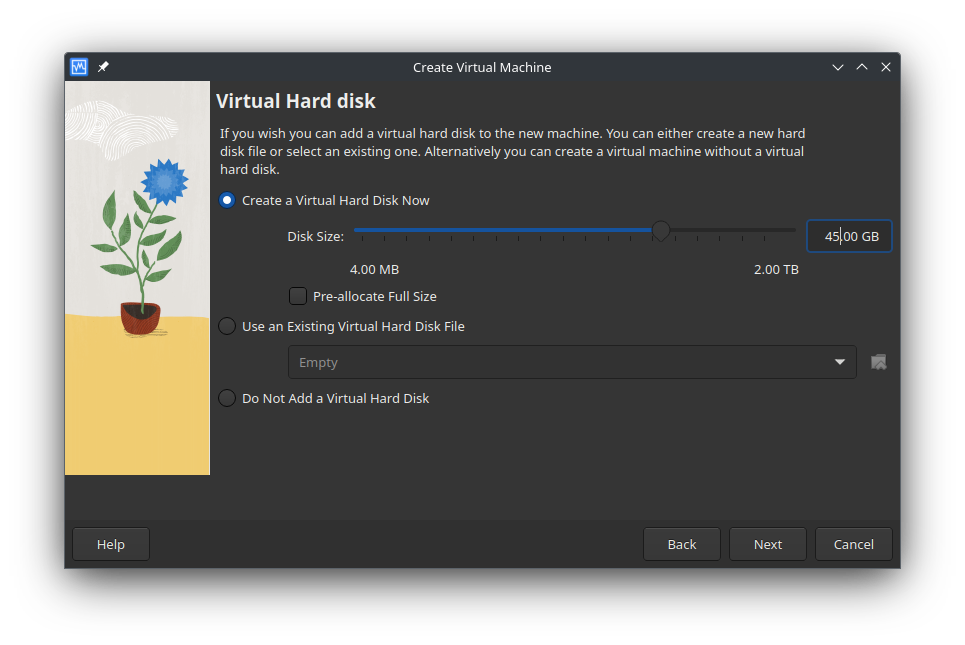
\includegraphics[width=\textwidth]{1-7.png}
\end{figure}

Make sure that the ``Create a Virtual Hard Disk Now" option is selected and set your desired amount of space. Here, I have chosen to allocate 45 GB of space.

Leave the ``Pre-allocate Full Size" box unchecked. This way, `empty' space in the Ubuntu install will not take up space on your actual hard drive.

Click ``Next".

\pagebreak

View the summary, ensure all details are correct, and click ``Finish" to create the virtual machine\footnote{The correct configuration options might differ slightly from this screenshot; namely, you need to set Skip Unattended Install to `true'.}.

\begin{figure}[htp]
    \centering
    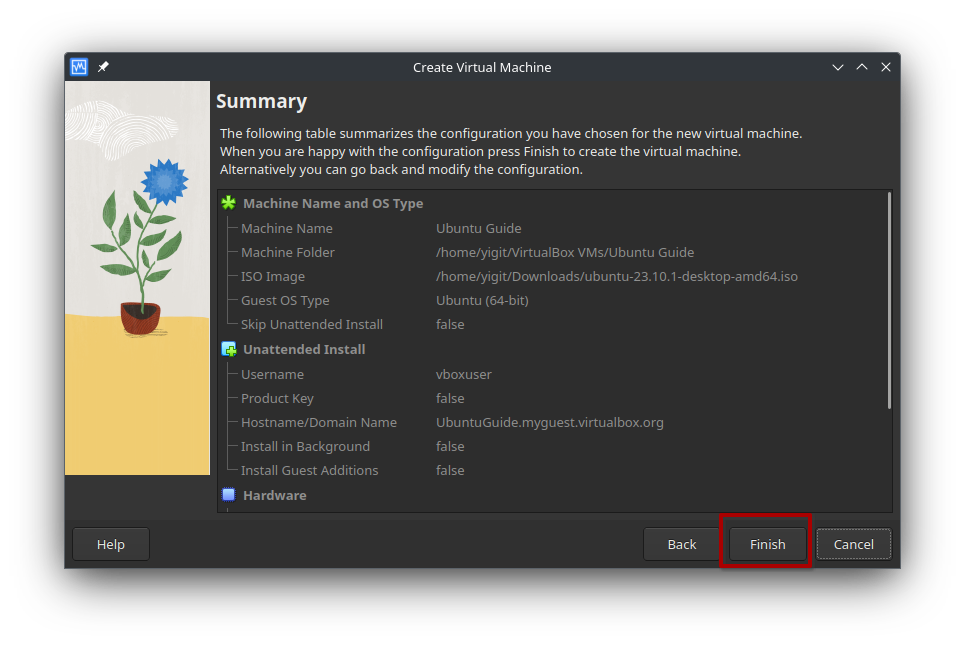
\includegraphics[width=\textwidth]{1-8.png}
\end{figure}

\pagebreak

If the installation went well, there is now a new entry in the VirtualBox main menu: 

\begin{figure}[htp]
    \centering
    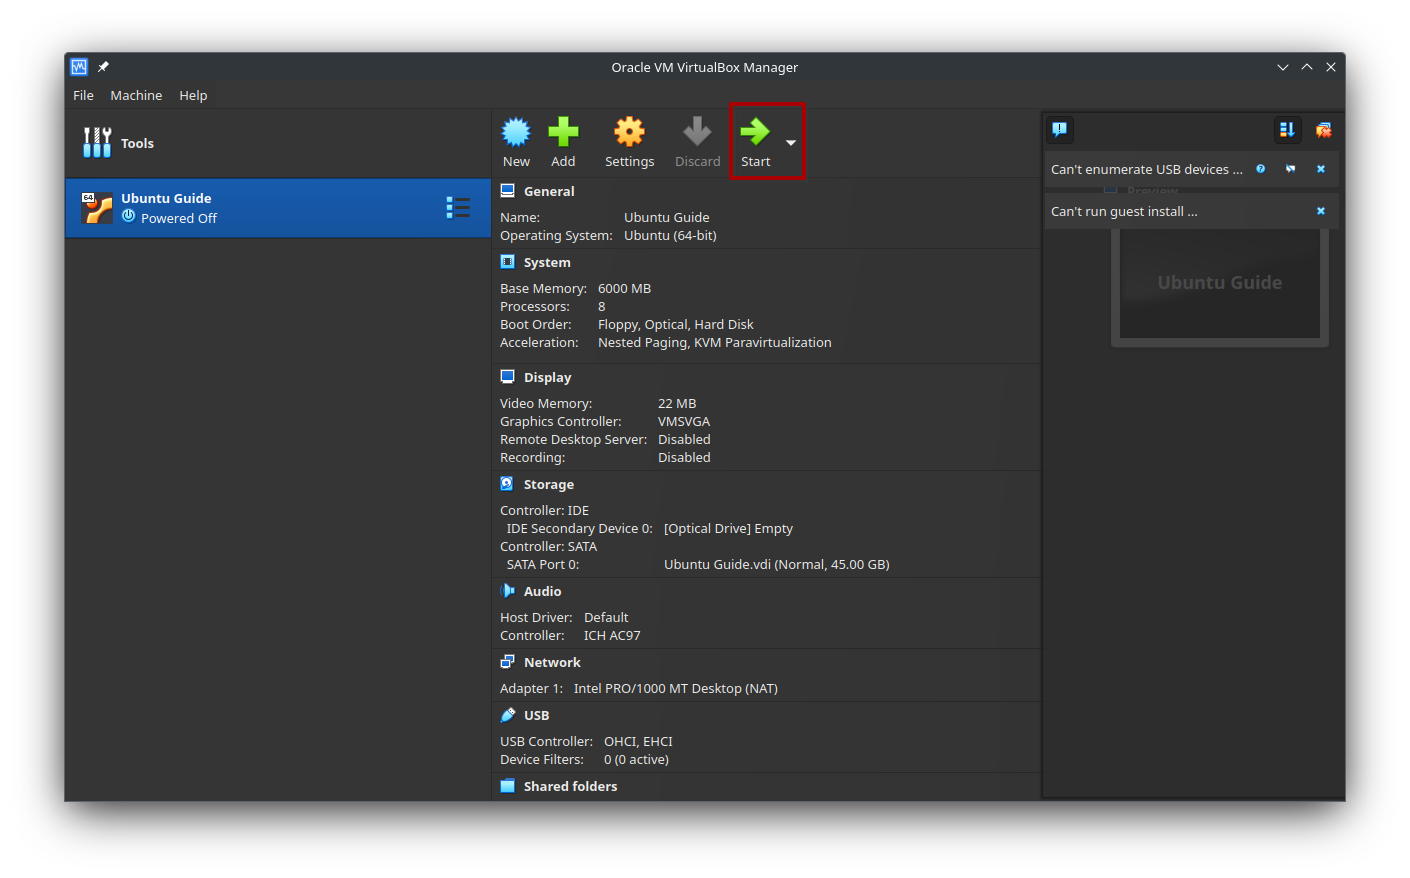
\includegraphics[width=\textwidth]{1-9.png}
\end{figure}

Click ``Start" while the new VM is selected to start the Ubuntu install process\footnote{If you see a message saying that the virtual machine failed to boot, point the ``DVD:" field in the pop-up box to the Ubuntu installation ISO. You can do this by clicking the drop-down arrow on the right-hand side of the field and choosing the ISO file from the menu. If the ISO file is not listed, click ``Other..." and then navigate to the ISO file in the file picker dialog.}.

\pagebreak

On the next screen (titled ``GNU GRUB"), make sure the ``Try or install Ubuntu" option is highlighted and press ENTER on your keyboard.



\begin{figure}[htp]
    \centering
    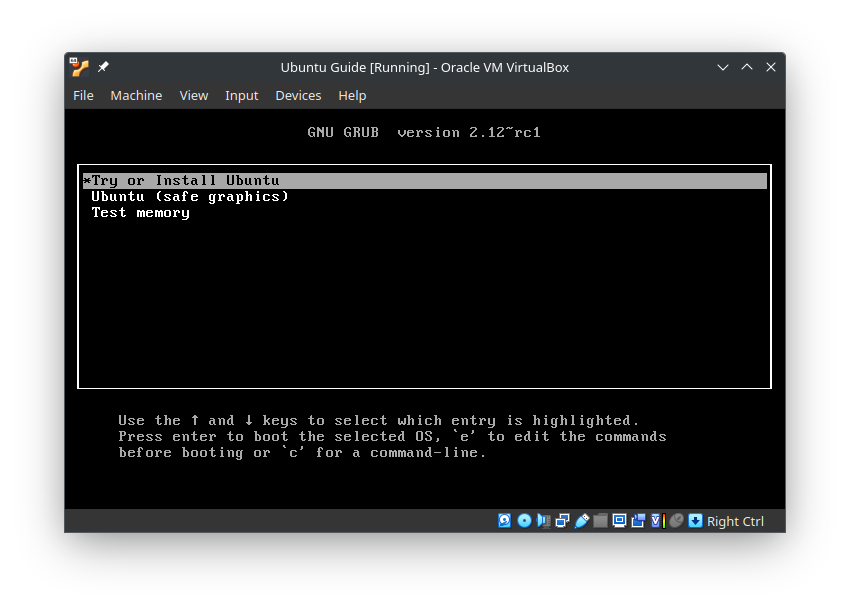
\includegraphics[width=\textwidth]{1-10.png}
\end{figure}


A loading screen will appear. It will take a bit of time for the installation medium to boot up.


%\begin{figure}[htp]
%    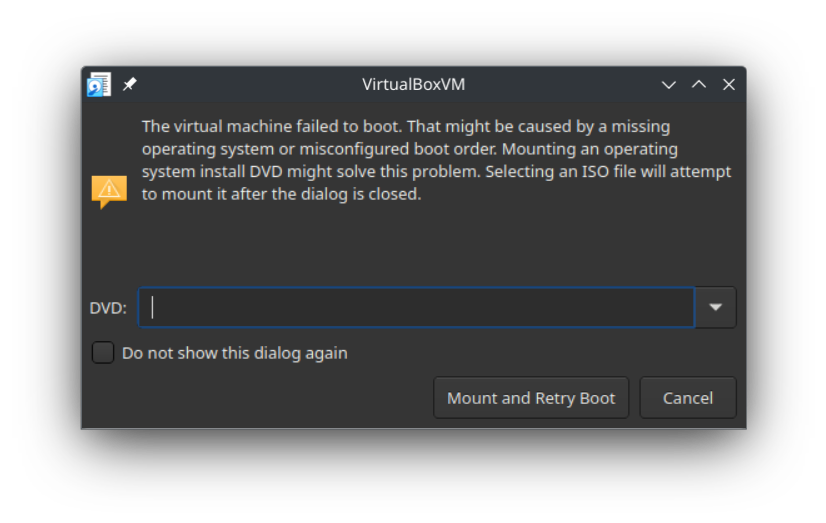
\includegraphics[width=0.8\textwidth]{1-12.png}
%    \captionsetup{labelformat=empty}
%    \caption*{If you see a message saying that the virtual machine failed to boot, point the ``DVD:" field in the pop-up box to the Ubuntu installation ISO. You can do this by clicking the drop-down arrow on the right-hand side of the field and choosing the ISO file from the menu. If the ISO file is not listed, click ``Other..." and then navigate to the ISO file in the file picker dialog. }
%\end{figure}

\pagebreak

If all goes well, the Ubuntu installation image will boot and you will see the Ubuntu setup dialog.

\begin{figure}[htp]
    \centering
    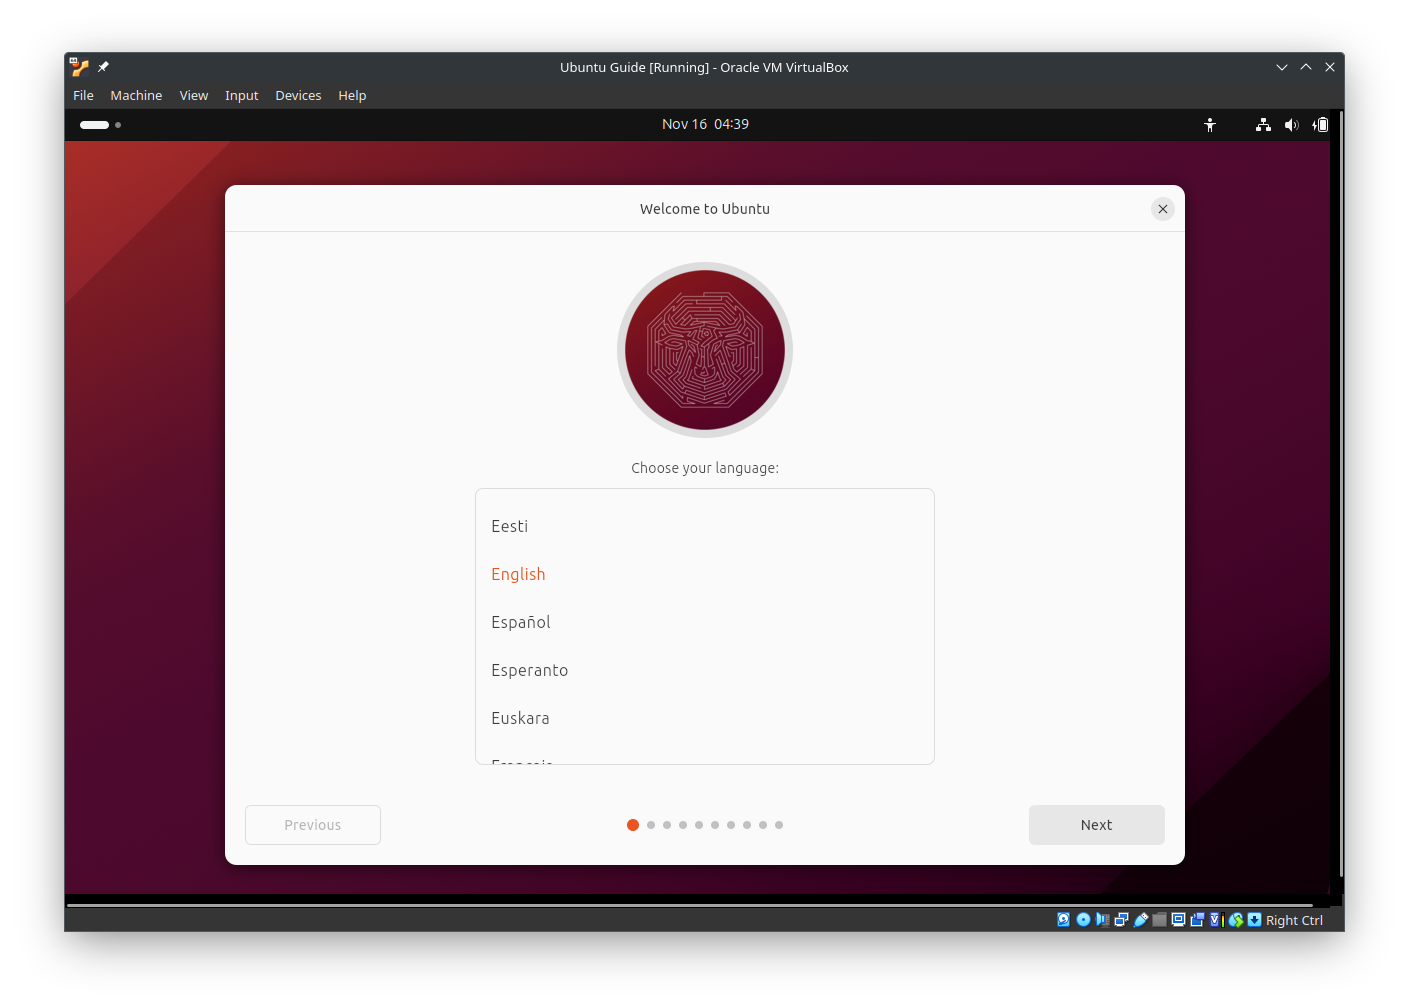
\includegraphics[width=\textwidth]{1-11.png}
\end{figure}

In the following screens, do the following:
\begin{enumerate}
    \item Select a language of your choosing. In this guide, we will select English.
    \item Select ``Install Ubuntu". Since we are installing Ubuntu into a virtual machine, we do not need to worry about data loss\footnote{If you are installing Ubuntu directly onto a hard drive, the ``Try Ubuntu" option will let you try out Ubuntu within the installation medium, but you will lose all changes you made when you reboot.} and thus can simply install Ubuntu without needing to try it out first. 
    \item Select your keyboard layout as desired.
    \item Select ``Use wired connection".
    \item You can skip the prompt to update the Ubuntu installer.
    \item On the ``Applications and updates" screen, select ``Default installation" (you will figure out how to install additional apps soon enough). I would recommend checking the two boxes in the ``Other options" section.
    \item On the following screen, select ``Erase disk and install Ubuntu" - this will wipe the (currently empty) virtual machine drive and install Ubuntu into it\footnote{The ``Manual partitioning" option allows you to customize your install, install Ubuntu alongside Mac OS or Windows, and so on. However, there are a lot of configuration options involved, so skip this step unless you are trying to install Ubuntu on bare metal.}.
    \item On the ``Ready to install" screen, check that the text under ``Devices" is \verb|VBOX HARDDISK sda| and then click ``Install". 
    \item Select your timezone.
    \item Fill the fields in the next step however you wish. The first field corresponds to the name you will see on the lock screen and so on. I have decided to use \verb|Ubuntu Guide|. 
    \item Decide on your computer's name. ``Your computer's name" is also called the \textbf{hostname,} and it is the name that your computer will have on the local network (e.g. over Bluetooth). Your hostname should have no spaces. I chose \verb|UbuntuGuide|.
    \item On the same screen, decide on a username - for convenience, this should be a short and all-lowercase name. You will use this username repeatedly in commands. I chose \verb|ubuntuguide|.
    \item Afterward, on the same screen set a password, confirm the password, and ensure that ``Require password to log in" is enabled. Move on to the next screen.
    \item Choose a theme on the next screen.
    \item Ubuntu will now be installed into the virtual machine you have created. Once the confirmation screen appears, click ``Restart now" to reboot the VM into Ubuntu proper.
    \item Remove the install medium (from VirtualBox menu, navigate to Devices -\> Optical Drives, uncheck the Ubuntu ISO file) when prompted, and press ENTER.
    \item Wait until the VM reboots into the Ubuntu login screen.
\end{enumerate}

\begin{figure}[htp]
    \centering
    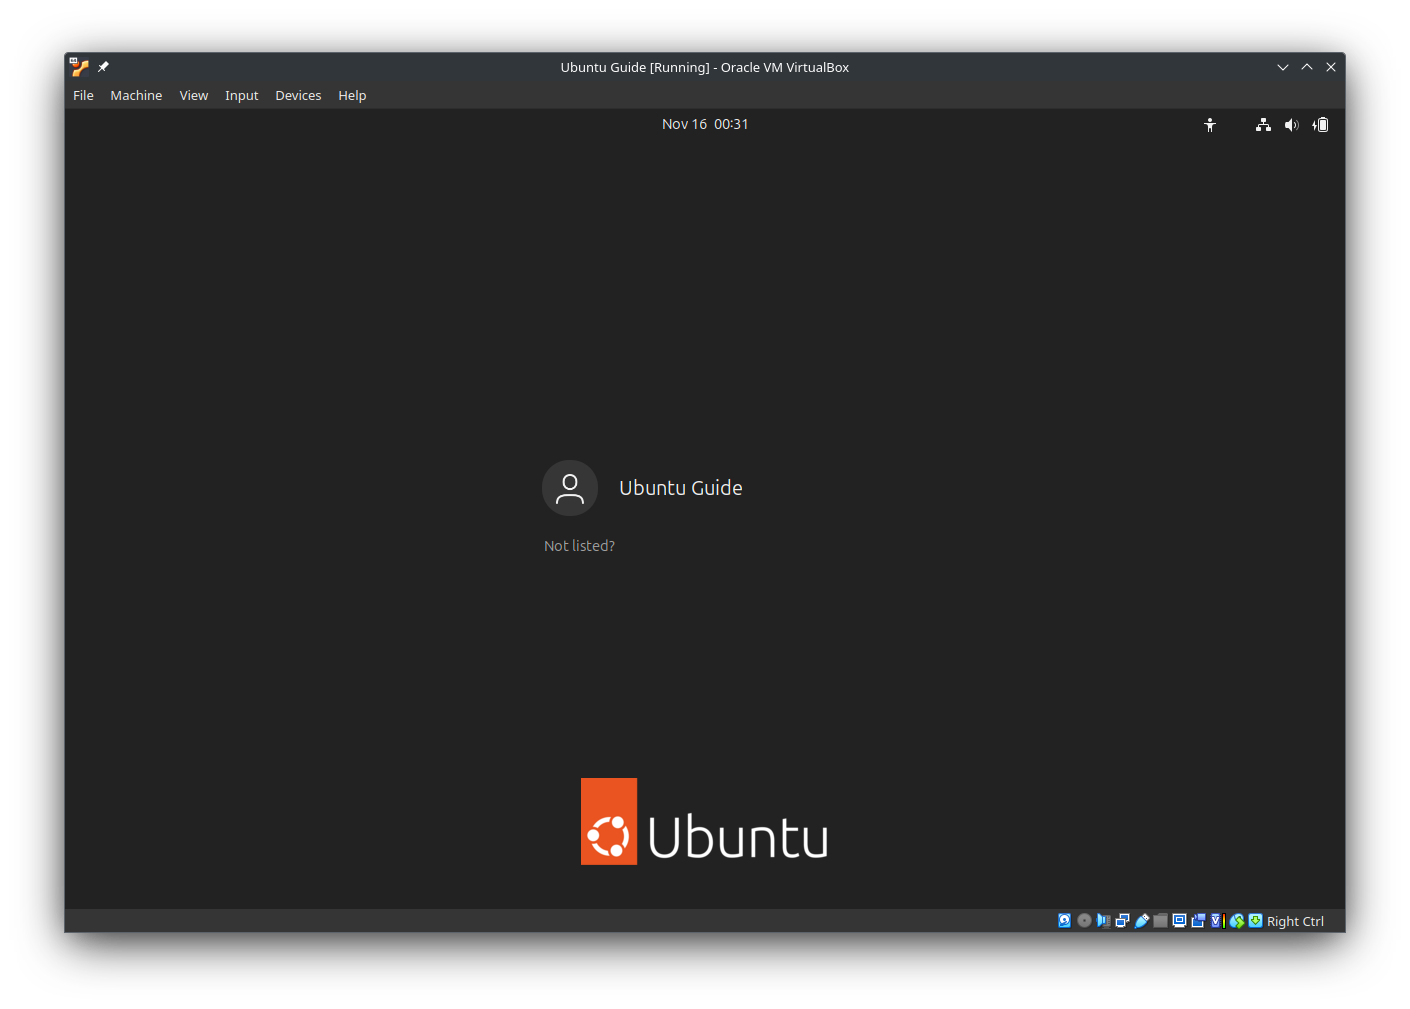
\includegraphics[width=\textwidth]{1-14.png}
\end{figure}

Congratulations! You have installed Ubuntu.

\pagebreak
\section{Ubuntu Basics: Getting Our Bearings}

And we are off!

\begin{figure}[htp]
    \centering
    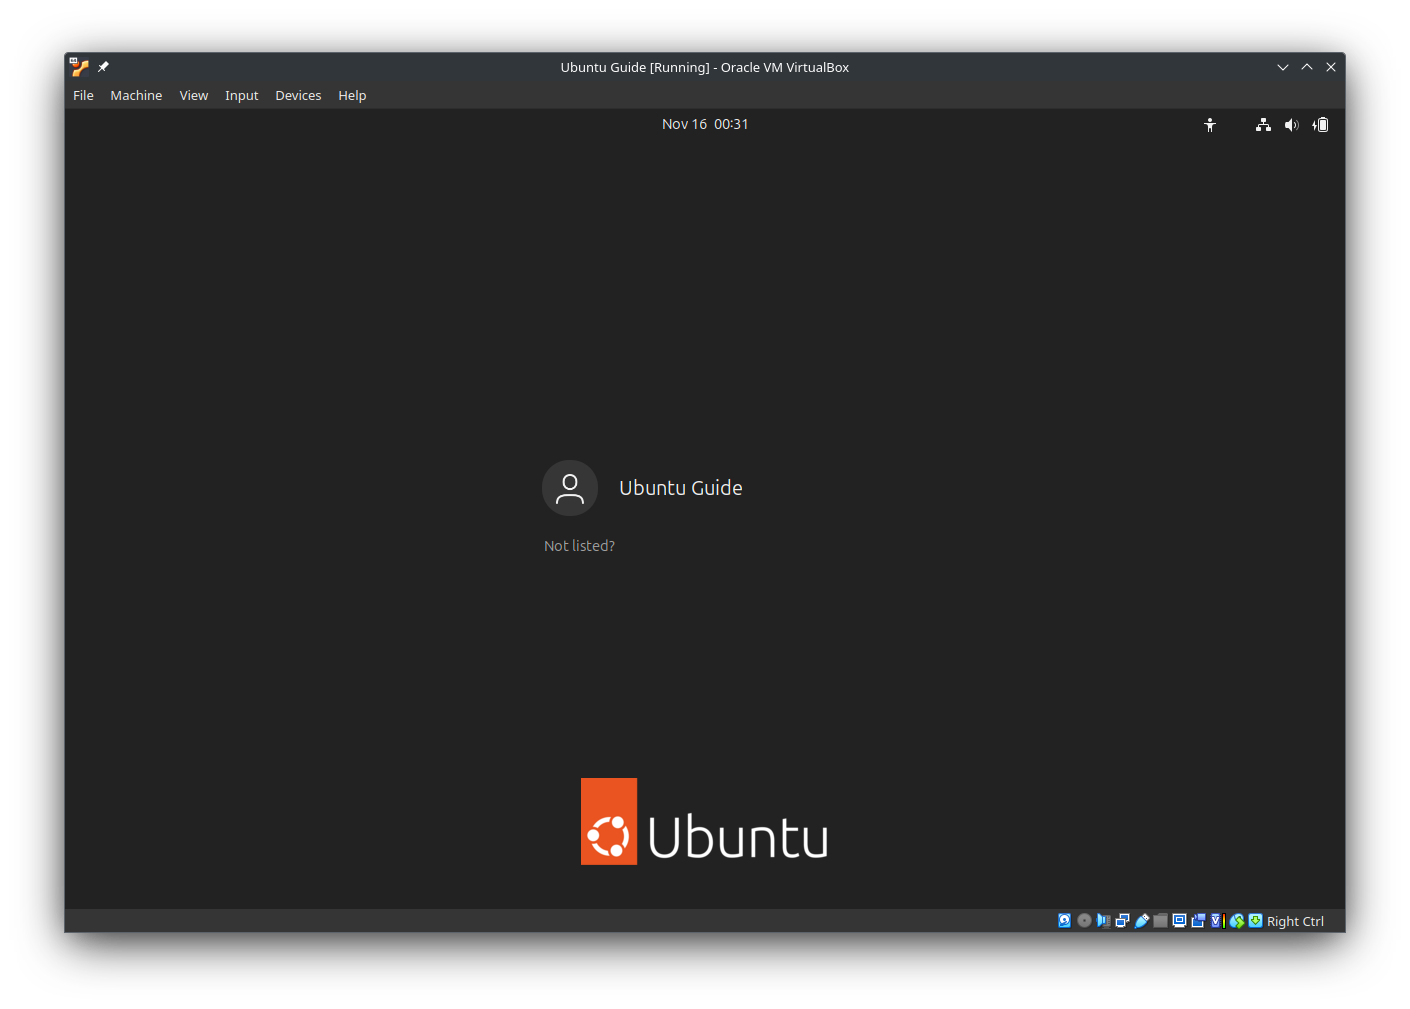
\includegraphics[width=\textwidth]{1-14.png}
    \caption*{The Ubuntu 23.10 login screen.}
\end{figure}

The lock screen in (default) Ubuntu is called the GNOME Display Manager, or GDM for short.

Click your name, input your password and press ENTER.

You will now log in to Ubuntu.

\pagebreak

\subsection{Where am I? - The GNOME Desktop Environment}

After a successful login, you will come across this screen:

\begin{figure}[htp]
    \centering
    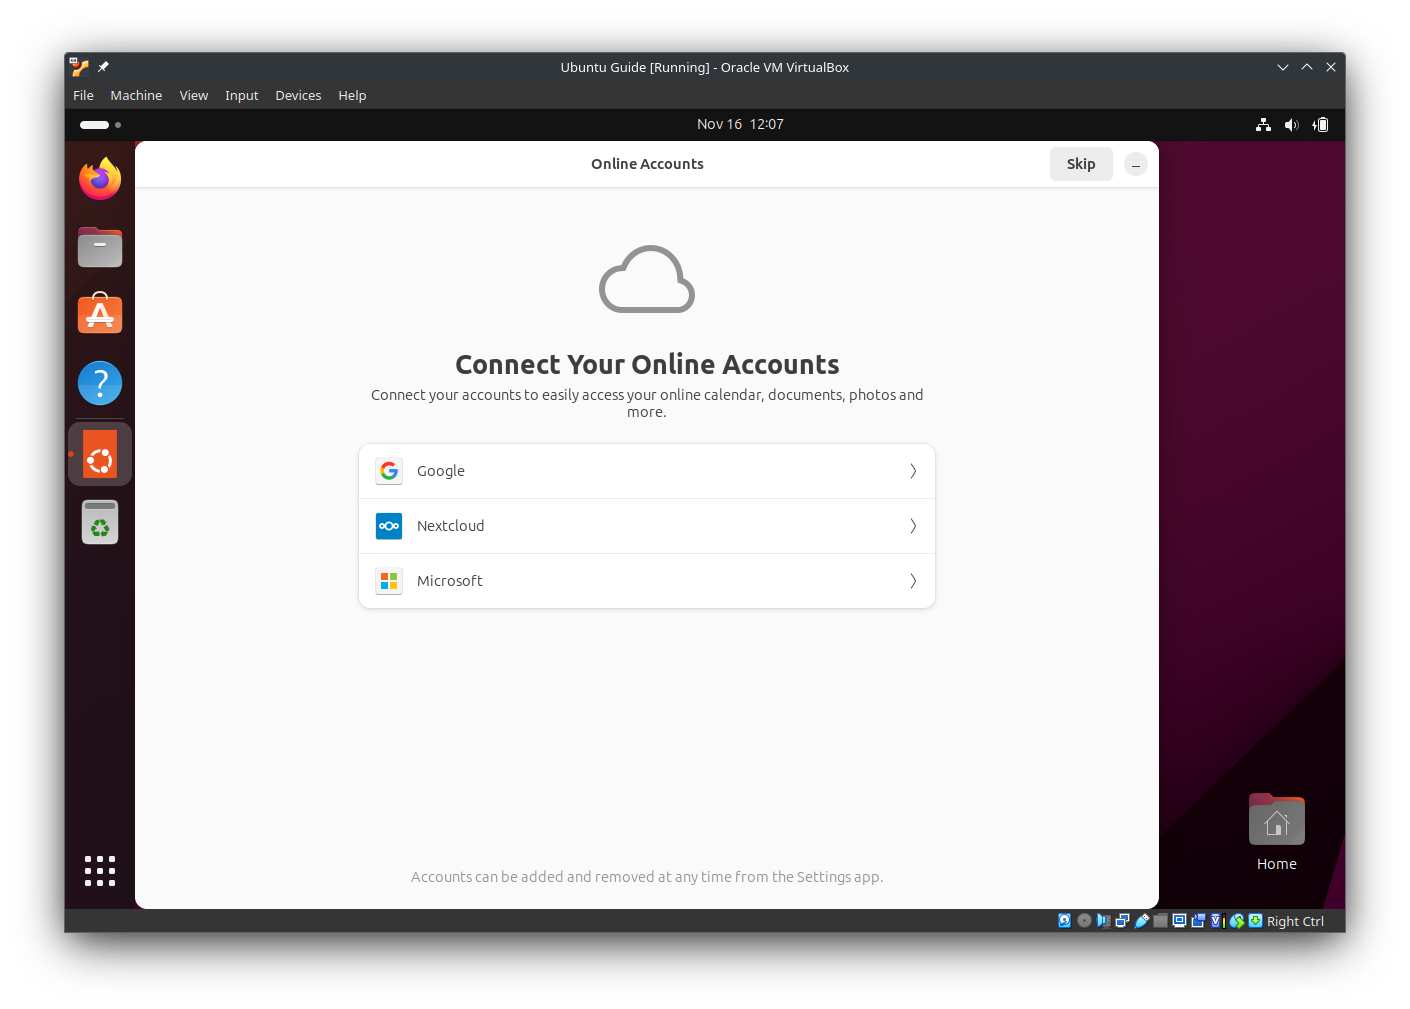
\includegraphics[width=\textwidth]{2-1.png}
\end{figure}

Close the white window by clicking ``Skip'' on the upper right corner of the window, then ``Next'', and finally ``Done''.

What you are looking at is called the \textbf{GNOME Desktop Environment}, or \textbf{GNOME} for short. 

Every visual element you see in the picture (besides the VirtualBox window borders) is a part of GNOME; from the taskbar on the left, to the desktop, to the thin bar at the top. \vspace{5mm}

\textbf{Sidebar:} There is an important but unintuitive - and uniquely Linux! - fact to take note of here: \textit{GNOME is actually distinct from Ubuntu!} Ubuntu itself is more so the \textit{backend} of your computer, GNOME is the thing determining what Ubuntu \textit{looks like.} Other distros can also use GNOME as their desktop environment, in which case they look very similar to this screenshot; conversely, Ubuntu can use other desktop environments and look completely different \footnote{Ubuntu supplies the GNOME desktop environment (DE) by default, which is why we are using GNOME right now. However, there are versions of Ubuntu that ship with \textit{different} desktop environments - Kubuntu ships with KDE Plasma, Ubuntu MATE ships with the MATE desktop environment, and so on.}.
\vspace{5mm}

Let's look at the primary UI elements on this screen.

\begin{figure}[htp]
    \centering
    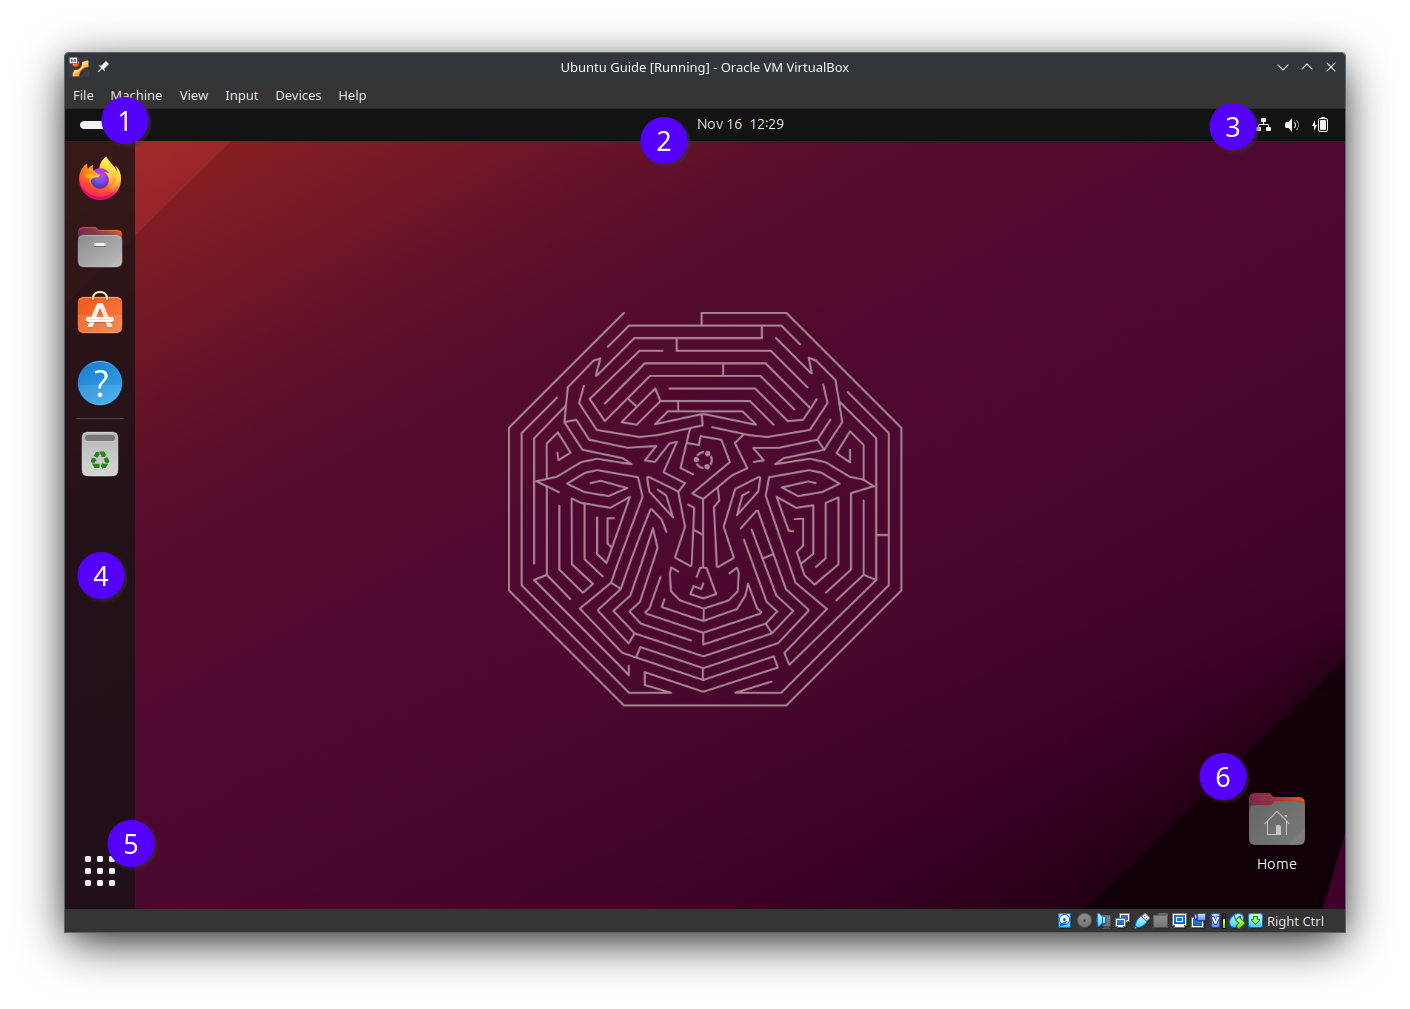
\includegraphics[width=\textwidth]{2-2.png}
\end{figure}

\begin{enumerate}
    \item \textbf{Activities button:} Click this corner of the screen to go to the Activities view, where you can view all workspaces at once. The ellipse shows you which workspace you are currently viewing (circles denote other workspaces). Pressing the \textbf{SUPER key} (Windows key/ Option key) has the same effect.
    \item \textbf{Top bar:} This top bar features a clock, the Activities button (left), and the system status area (right). 
    \item \textbf{System status area:} View system information (e.g. battery level) here. You can access the \textbf{user menu} by clicking the system status area; the user menu has options for common system settings like Wi-fi, Bluetooth, and power-off options.
    \item \textbf{Dash:} This is where you can view the currently open applications and launch them, usual desktop fare.
    \item \textbf{Application launcher:} Click this button to bring up the application launcher (a grid of desktop applications).
    \item \textbf{Desktop icons:} As usual, the desktop houses shortcuts to various folders and programs. You do not really need to use this often in GNOME, though; the application launcher and Activities overview are better-integrated tools for finding files, folders or apps.
\end{enumerate}

If you press the SUPER key (that's the Windows key on Windows computers or the ``option" key on Mac) or click the upper-left corner on this main screen, you will get to the Activities overview.

\begin{figure}[htp]
    \centering
    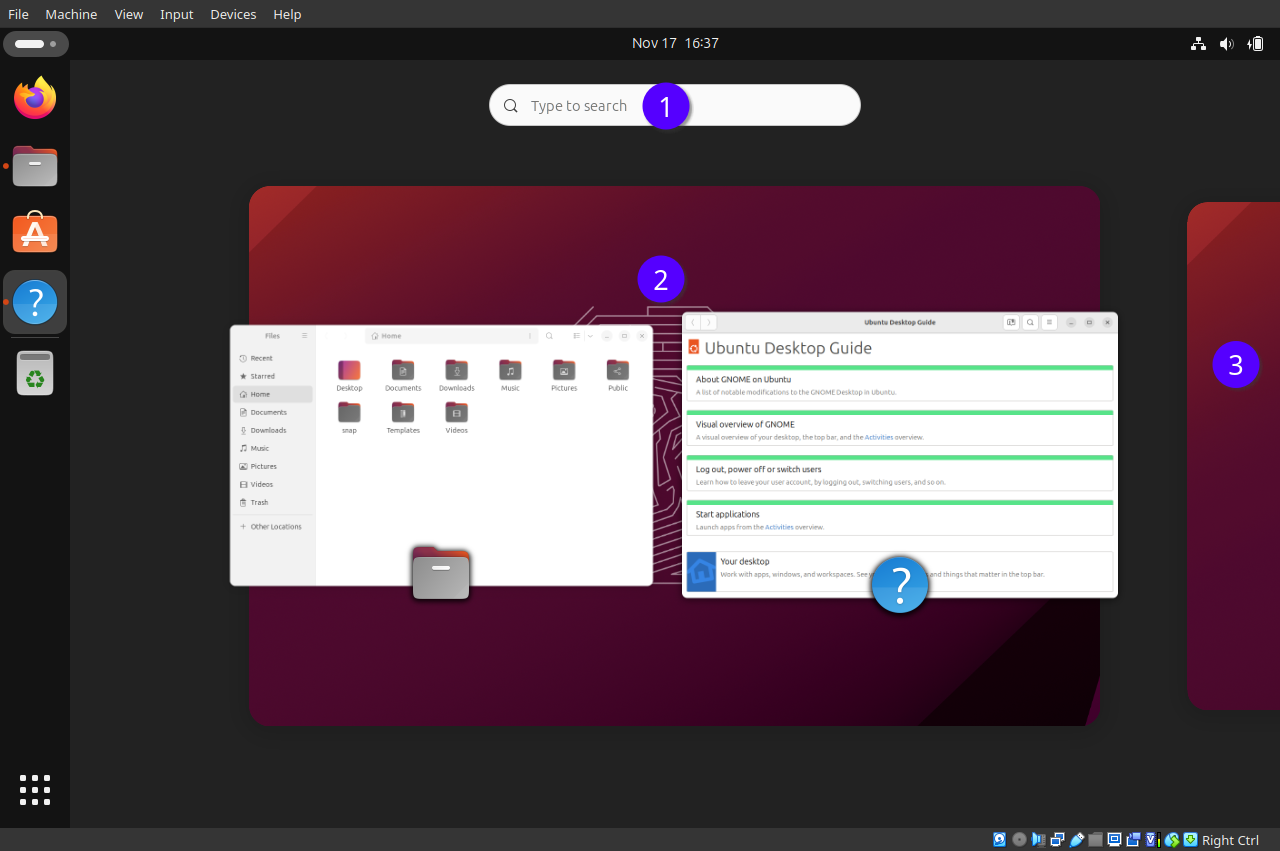
\includegraphics[width=\textwidth]{2-3.png}
\end{figure}

I opened a couple windows (``Files'' and ``Help" from the Dash on the left side) to illustrate how this screen looks when you have a few windows open.

Here are the key features of this screen:

\begin{enumerate}
    \item \textbf{Search bar:} You can launch applications quickly from here by starting to type their name - a list of results will show up as you type. You do not need to click the search bar to start a search - you can just start typing.
    \item \textbf{Window overview:} You will see all windows open in the current \textbf{workspace} in the middle of the screen. Generally, you will use workspaces to group various windows, as they act like different desktops you can quickly switch between. Scroll with your mouse or touchpad to focus on different workspaces.
    \item \textbf{Next workspace:} You can see the (currently empty) second workspace on the right-hand side. If you are working with multiple workspaces, there might also be another workspace on the left. If you drag and drop a window into this area, it will move to this workspace.
\end{enumerate}

The overview is important because it will be a key part of your workflow in GNOME. The best way to figure out how it might be useful for you is to spend some time working in it. 

It is worth noting that the overview deliberately discourages relying on desktop icons, unlike Windows (and arguably Mac). Once you adapt, it'll be quicker and easier to launch apps by going into the overview and typing their name, compared to looking for a desktop shortcut each time. 

\pagebreak

\subsection{The Terminal}

In order to understand how to effectively use Linux, you will need to learn how to use the terminal. 

From the GNOME desktop, open the application menu or the overview, and search for `Terminal'. This is the most important program in Ubuntu.

Launch the terminal by clicking the Terminal icon, or pressing ENTER.

\begin{figure}[htp]
    \centering
    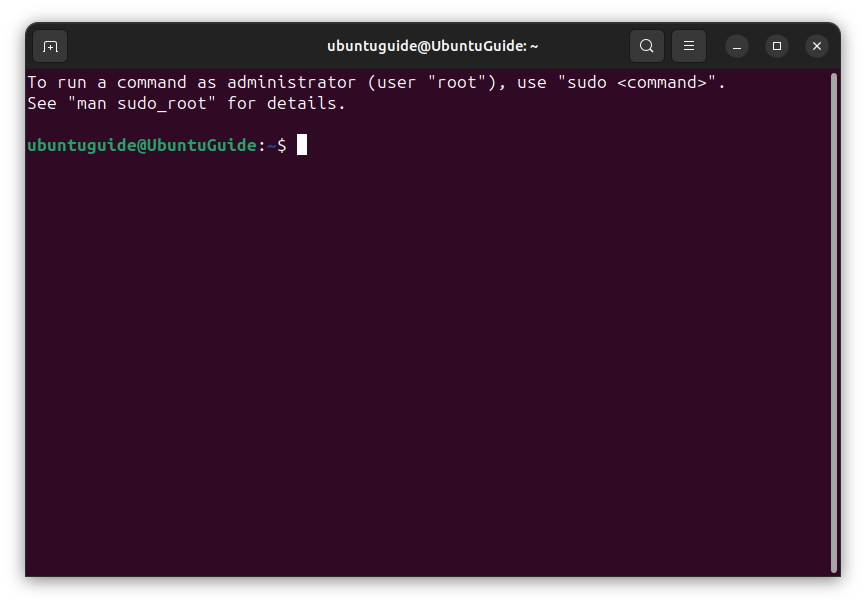
\includegraphics[width=\textwidth]{2-4.png}
\end{figure}

This is the terminal. The central idea is simple- you give the computer a text command, and the computer does what you say. 

You can use the terminal to do \textit{just about anything-} you can code, manipulate files, install or start programs, change your computer's settings, play music... Essentially, the terminal is a whole new way to use your computer. In the rest of this section, I will introduce you to some basic concepts about the terminal and show you a few basic terminal commands.

\subsubsection{Terminal basics}

The types of programs you are used to running, which create a window and have visual elements you can then interact with (using a mouse and keyboard), are called \textbf{Graphical User Interface (GUI)} programs. 

In contrast, the programs you run in a terminal by issuing text prompts are called \textbf{Command Line Interface (CLI)} programs. These programs take text as input, and often have text as output; however, they can also create, modify and delete files much like GUI programs.

Let's look at an empty terminal.

\begin{figure}[htp]
    \centering
    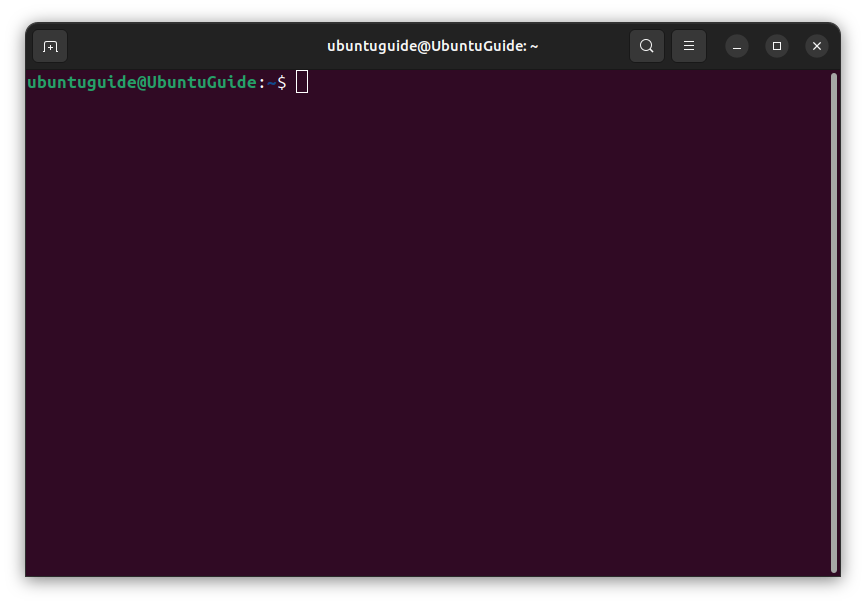
\includegraphics[width=\textwidth]{2-5.png}
\end{figure}

The colorful text at the start, \verb|ubuntuguide@UbuntuGuide:~$|, is called the \textbf{command prompt.} The command prompt tells you which user you are logged in as, which machine you are logged in to, and where you are in the file system of this machine. Let's dissect it:

\begin{itemize}
    \item \verb|ubuntuguide| is our \textbf{username.} You will use your username for a lot of things - this is basically the name the Ubuntu knows you by.
    \item \verb|@| separates the username from the hostname. Conventionally, the username is all lowercase.
    \item \verb|UbuntuGuide| is our \textbf{hostname.} This is the name that the Ubuntu installation will show to other devices on the network. Essentially, this is the name of the machine. Conventionally, the host name is one word but can include capital letters.
    \item \verb|:| just separates the hostname from the current directory - see below.
    \item \verb|~| is the \textbf{current working directory.} This is your location in the file system. The tilde (\verb|~|) is shorthand for your \textbf{home directory-} that is to say, \verb|~| here is equivalent to \verb|/home/ubuntuguide|. You will learn more about how Linux organizes system files and how to navigate a Linux file system in the terminal later on. 
    \item \verb|$| indicates the end of the command prompt. Furthermore, the fact that this icon is \verb|$| tells us that we are currently logged in as a non-administrator. The administrator account (called the \textbf{root account} in Linux parlance) has a slightly different command prompt which ends in \verb|#| instead of \verb|$|.
 \end{itemize}

 \pagebreak
\subsubsection{echo}

The first command we will learn about is \verb|echo|. This command basically prints out the text\footnote{Text strings are usually enclosed in single or double quotes. There IS a difference between using double and single quotes, but you do not need to worry about that at present.} you put in without changing it.

Give it a try: Type \verb|echo "Hello World"| in the terminal, and press ENTER.

\begin{figure}[htp]
    \centering
    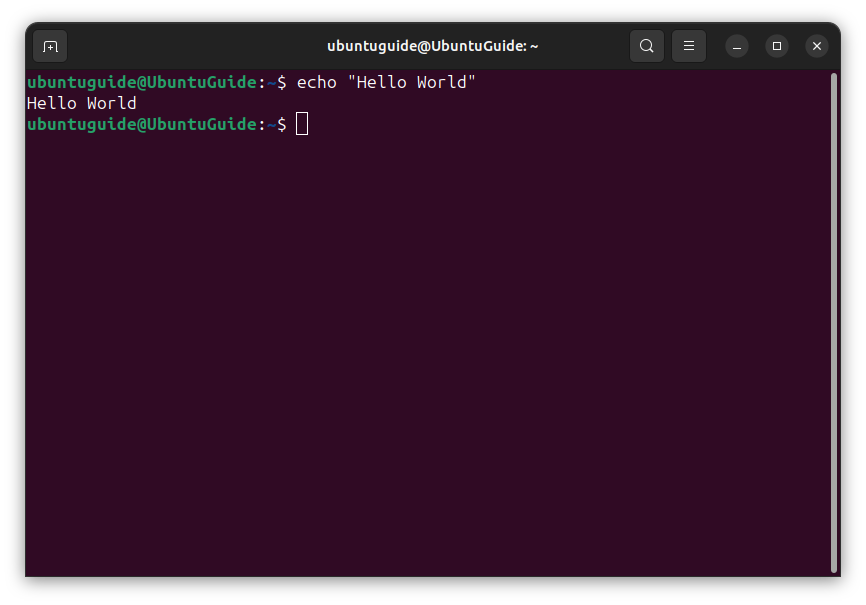
\includegraphics[width=\textwidth]{2-6.png}
\end{figure}

Congratulations! You have just run your first terminal program. 


\end{document}